\chapter{Visualization Layer}\label{viz-ch}

The primary function of the visualization layer is to render a spectrogram
served by the compute layer. In addition, this module is responsible for
providing a usable interface for an analyst to work with the datasets.
Minimizing latency is an important design goal since increased latency can
dramatically reduce an analyst's efficiency if they must continually wait for
the interface to respond from their queries. \\

We chose to build browser based visualizations since they allow ease of use for
an analyst, who only has to visit a webpage instead of installing any software
aside from the browser itself.  Also, the analyst does not require special
hardware since the intensive storage and computations are handled by the
server. This choice makes the job of visualizing interactively more difficult
since the browser is much more limited in network bandwidth and rendering
capabilities compared to a native application. (add sources to back this up, or numbers)

\section{Design}

\subsection{Interface}

The interface should provide the analyst with the ability to specify a patient
\c{mrn} to query, a \c{start\_time} and \c{end\_time} and also afford quick
navigation between time ranges. The workflow that we anticipate is that an
analyst will load a single patient file and browse subsequent time frames. If
an interesting section is reached, the analyst should be able to zoom in to see
further details. The interface should also give the analyst information about
the visualization, such as interactive axes. The interface should also provide
user feedback for errors, cleaning data on the client to prevent inadvertent
queries from being issued.

\subsection{Communication}

Optimizing communication is important to avoid creating a bottleneck that can
affect latency. The point which is most likely to be a bottle neck is
deserializing the data received from the network.

\subsection{Rendering}

The client rendering must be able to efficiently render large matrices of
floating point values, on the order of several million points. Some amount of
data aggregation is acceptable, for example downsampling, however the overall
data quality must not be degraded when presented to the analyst.

\section{Implementation}

The visualization layer is implemented primarily using HTML, JavaScript and
CSS. Rendering is done via WebGL to take advantage of the client GPU. The
implementation has been tested and evaluated with Chrome (46.0.2490.86) and
Firefox (42.0) on OSX 10.11.1 and Ubuntu 14.04. (get swang's version of
chrome/FF).

\subsection{Interface}

The interface is shown in Figure \ref{fig:whole-interface}. This interface
shows a sample of the patient \c{005} being rendered between the second and
third hour of the scan. These parameters are specified in the top bar with the
ability for the analyst to scroll to previous or next hour with a single click.
The scrolling interval defaults to 1 hour, but is configurable in the settings
window. \\

\begin{figure}[h]
\begin{center}
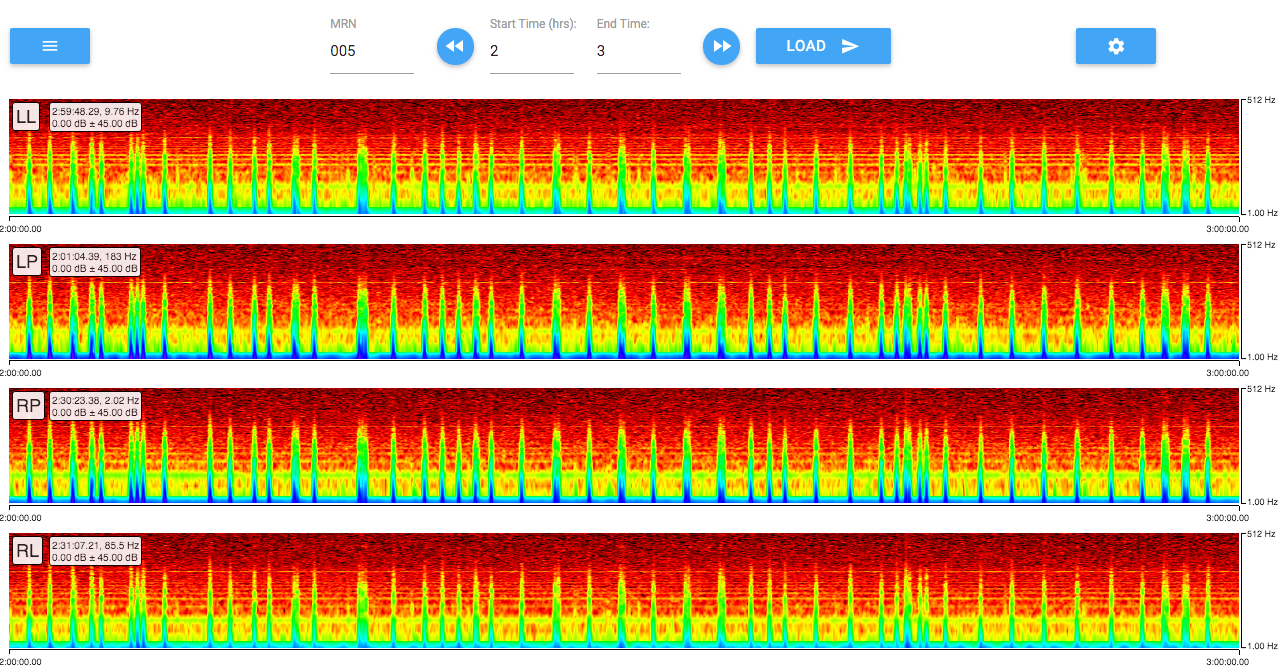
\includegraphics[scale=0.35]{./img/whole-interface.png}
\caption{Screenshot of Pinky's user interface.}
\label{fig:whole-interface}
\end{center}
\end{figure}

Settings are accessed by clicking the small gear on the far right of the
interface and the options are shown in Figure \ref{fig:settings}. The settings
page allows an analyst to change the rendering mode, time interval and select
options for interpolation and the visualization scale. In addition, there are
two keyboard shortcuts which allow an analyst to change the amplitude scale or
zoom in on the visualization. Figure \ref{fig:zoomed-region} shows the result
of a single region when a user zoomed in. \\

\begin{figure}[h]
\begin{center}
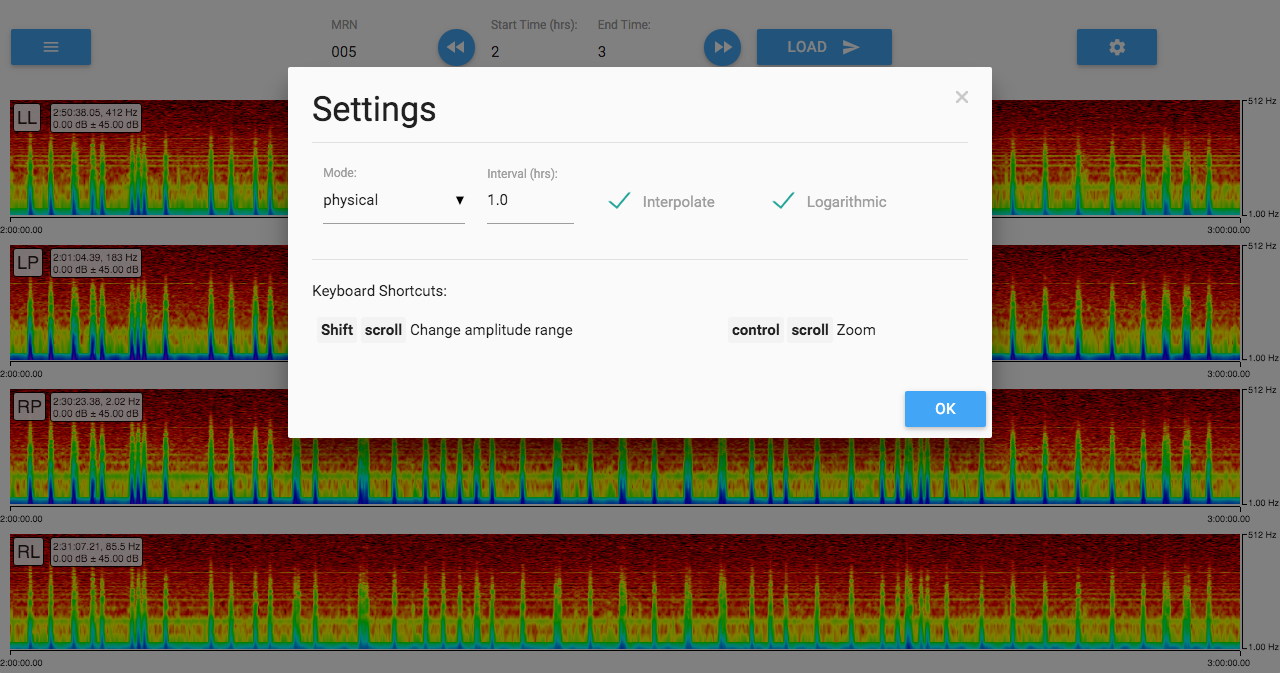
\includegraphics[scale=0.35]{./img/settings.png}
\caption{Screenshot settings modal.}
\label{fig:settings}
\end{center}
\end{figure}

The interface shows a spectrogram for each region of the brain, each region is
label in the upper left hand corner with \c{LL}, \c{LP}, \c{RP}, or \c{RL}.
Next to these labels, as can be seen in Figure \ref{fig:zoomed-region} is a
small box containing axis information, specifying where the user's mouse
currently is. In this box the current timestamp (x-axis) and frequency (y-axis)
are show. In addition, the current amplitude value in dB is given as well as
the current amplitude viewing range. \\

\begin{figure}[h]
\begin{center}
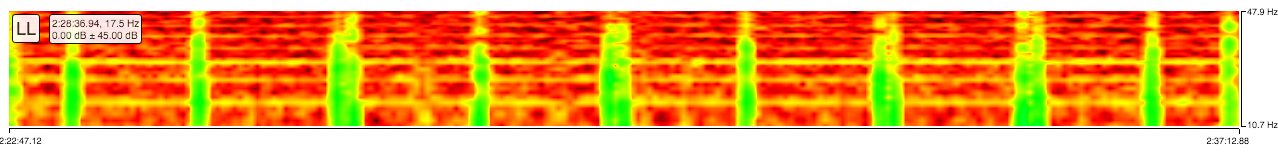
\includegraphics[scale=0.35]{./img/zoomed-region.png}
\caption{Screenshot of a zoomed in view of a single rendered region with
  dynamic axis labels.}
\label{fig:zoomed-region}
\end{center}
\end{figure}

While loading the interface blurs the spectrograms and presents a loading bar
to the user, as shown in Figure \ref{fig:loading}. This is done to
prevent confusion if there is a delay between the rendering of each region. If
a region is blurred and has a loading bar on it, it is clear that the new
region has not yet updated to the client's latest query. \\

\begin{figure}[h]
\begin{center}
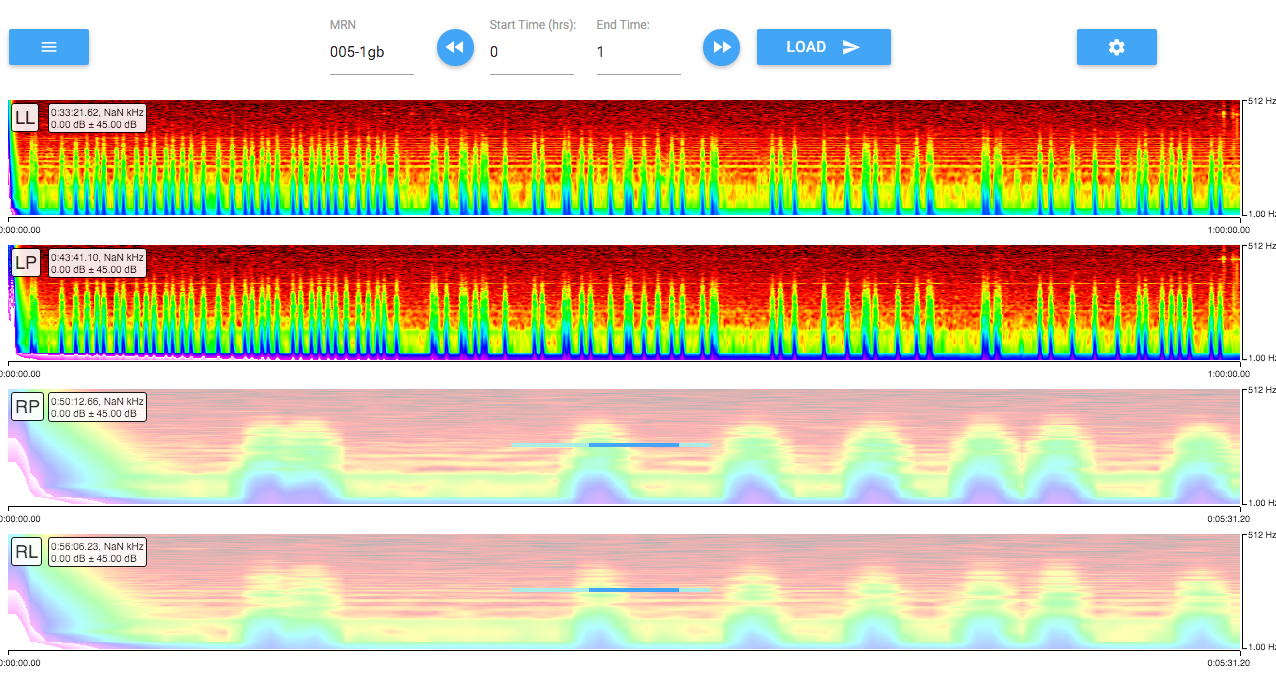
\includegraphics[scale=0.35]{./img/loading.png}
\caption{Screenshot of loading interface.}
\label{fig:loading}
\end{center}
\end{figure}

If an analyst enters an invalid \c{mrn}, the interface responds by clearing all
of the rendered spectrograms and displaying a small error message as shown in
Figure \ref{fig:error}. An invalid \c{mrn} is simply one which the
\c{StorageBackend} does not contain an array for. This could be from a user
error or when an array is currently being ingested into the system. This user
interaction is important to avoid analyst confusion if the display did not
update when the invalid query is issued. \\

\begin{figure}[h]
\begin{center}
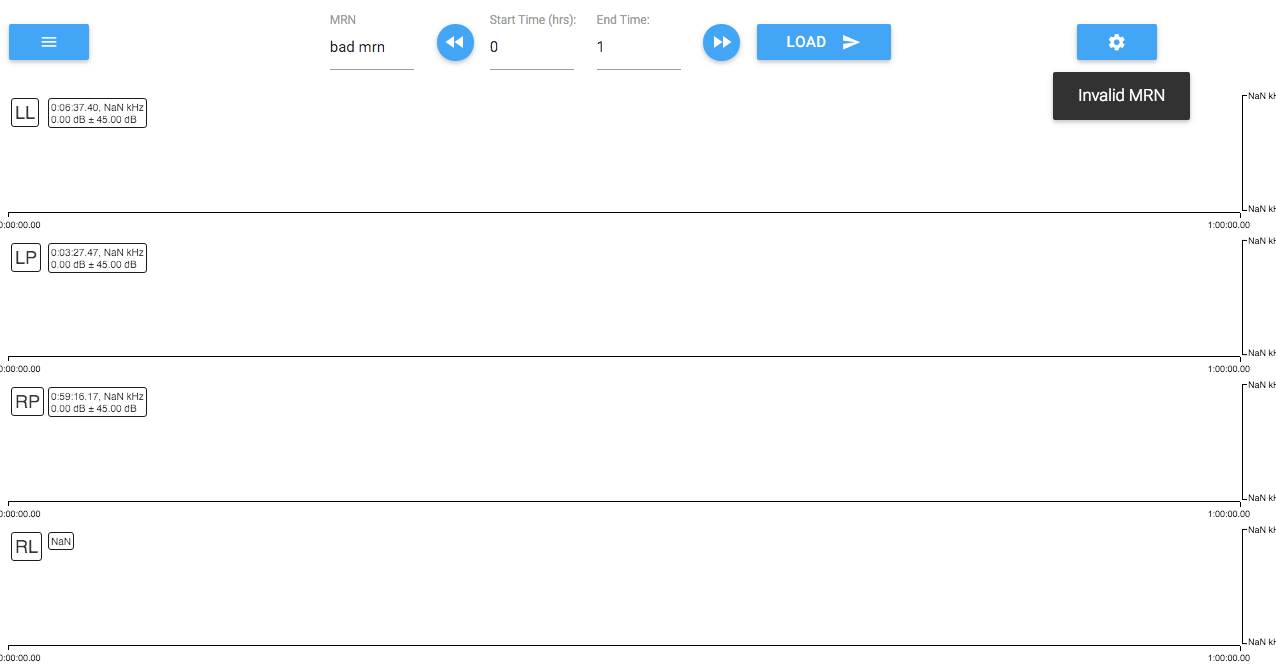
\includegraphics[scale=0.35]{./img/error.png}
\caption{Screenshot of error message for an invalid \c{mrn}.}
\label{fig:error}
\end{center}
\end{figure}

The materialize CSS library \cite{materialize} was used to layout the page
structure and keep a consistent style throughout the webapp.

\subsection{Communication}

Communication is primarily done via a websocket which is connected to the
compute later websocket server. Data requests are sent via JSON to the
websocket server and binary responses are decoded to extract the computed
spectrogram data for a given region. The binary protocol is described in
section \ref{compute-ch:implementation-ws-server}.

We make use of the reconnecting-websocket \cite{reconnecting-websocket} library
to ensure a smooth user experience is the analyst leaves the page long enough
for the connection to close.

\subsection{Rendering}

Rendering is completed use the Web Graphics Library (WebGL). WebGL is
JavaScript API which can render interactive 2D or 3D computer graphics without
the use of any third party plugins. The initial implementation is based on the
open-source library WebGL-Spectrogram \cite{webgl-spectrogram}. This library
has the functionality to render the spectrogram of an audio file from a
lightweight Python websocket server. We modified this library to a more general
version to contain multiple canvases, one for each brain region, and to
communicate with the compute layer websocket server. \\

\subsection{Optimizations}

WebGL was chosen since it is much more performant than using a browser's canvas
object or rendering DOM elements directly. Each spectrogram is an array on the
order of millions of points, we would not be able to achieve the latency
required for interactivity without the GPU rendering. Development time suffers
from the use of WebGL since it is difficult to understand the programming model
without some background in graphics rendering. In addition, we use JavaScript
typed arrays to transfer the binary data from the websocket to the GPU.
JavaScript typed arrays are array-like objects providing access raw binary
data. JavaScript engines optimize these arrays giving higher performance than
the traditional JavaScript \c{Array} object.

\section{Related Work}

